\section{Battery Management System}
INTRO HERE ------
The purpose of the Battery Management System (BMS)...
INTRO HERE ------

\subsection{Design}
In this paragraph a detailed documentation of the BMS' hardware will be given. Furthermore, each unit contained in the BMS will be described where the implementation and contents of each unit is viewed upon as a black-box. This means that the units will be considered purchased from a third party vendor and therefore a detailed description of the circuitry will not be given. This will lead to a different form of documenting with a lot of references to the "manufacturers" documentation that is the "BAC-projekt\_BMSogbatteri\_2013" \fxnote{Reference til dokumentationen / lokaliteten} documentation. Thus the general purpose and overview of each unit will elaborated in this section. 

\subsubsection{Propulsion battery}
Er flyttet til Hardware/Battery 

\subsubsection{Analog Front end}
The purpose of this unit is that it performs calculations and analog to digital conversion of the battery's cell voltages, battery's temperature and the signal from current sensor. Moreover, this unit manages cell balancing on request from the digital unit. It also has additional battery protection independent of the digital unit.


\subsubsection{Current Sensor}
The purpose of this unit is to measure the amount of amperes flowing through it as well as the direction of the current. This data is handled by the Analog Front End.

\subsubsection{Isolation Switch}
The Isolation Switch has a very important function in the BMS. If anything goes wrong with the battery, which means it exceeds the safe operation area then the Isolation Switch will prevent any current from flowing to the distribution block.

\subsubsection{Digital Unit (HW)}
This unit's purpose is to gather the measured values from the Analog Front End and thereafter run calculations and approximations of cell and battery parameters. If any of these parameters exceeds a specific threshold then the Digital Unit is capable of utilizing the Isolation Switch to prevent damages to the rest of the vehicle's system. Furthermore the Digital Unit is capable of communication with external units. 


\subsection{Implementation}
text

\subsection{Unity test}
text

\subsection{Programming Quick Guide}
The purpose of this section is meant to help whoever is going to work with the BMS in the future. Here you will be guided in how to use, debug and program the Digital Unit.

Firstly, you will need a few prerequisites listed below to be able to program the BMS. Since the BMS was originally build in 2013 the software to program the BMS is outdated but sometimes it is only possible to proceed and get it to work with the specified utilities. 

Tools required to program the BMS are listed here:
	\begin{itemize}
		\item AVR Studio 4 (tested with version 4.19 Build 730).
		\item Atmel Studio 6 or 7 (Both tested).
		\item JTAG-USB programmer (programmer that is included with the BMS hardware).
		\item 2 batteries (used to power the BMS).
		\item Tera Term (or any other hyper terminal).
		\item USB-A to USB mini cable (used to debug the BMS and see readouts from Tera Term).
	\end{itemize}
	
After you have acquired these tools you are ready to proceed. First of you connect the USB cable from your computer to the BMS front end. Then you launch your chosen hyper terminal and select the COM-port which the BMS has. Afterwards you configure the hyper terminal, where the two most important settings are the baud rate and the way you receive from the BMS. Set the baud rate to 38400, 1 stop bit, 8 data bits and 0 parity bits. Then you specify the newline settings so that you receive both CR+LF else select AUTO. In Tera Term you go to Setup->Terminal->New-line to perform these changes. 
Now you can attach the two batteries to the BMS (remember to plug in both the main plug and the cell plug to the front end), once this is done you're ready to receive data from the front end and it should look something like in the figure below \ref{fig:BMSTeraTerm}.
\begin{figure}[H]
	\centering
	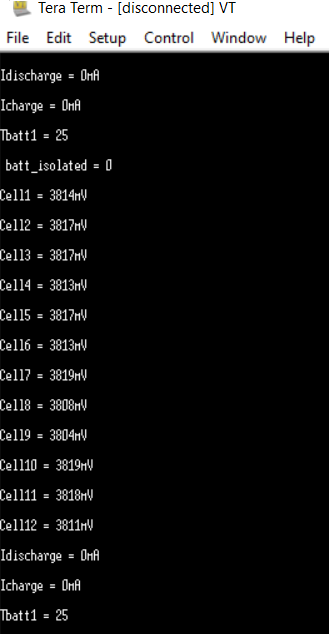
\includegraphics[width=0.6\linewidth]{Hardware/Pictures/BMS_teraterm}
	\caption{Tera Term Printout from BMS}
	\label{fig:BMSTeraTerm}
\end{figure}

Now you're ready to program the BMS. You can compile the code from either Atmel Studio 6 or 7, when you're done compiling you'll have a .hex file which is used for the AVR-CAN (Digital Unit). From this point on you have to follow the guide located in the pdf-file "How-to-install-and-use-AVR-JTAG-USB.pdf" which is located in the BMS repository. Now you can program the AVR-CAN module by selecting the .hex file or other valid files and program the BMS.

You can always confirm the programming by looking at the hyper terminal printouts and see if it matches your expectations. However, if it does not match your expectations you will have to debug the source code or the hardware to resolve the problem.

